% !TEX root = ./Basilisk-thrFiringRemainder-2019-03-28.tex


\begin{figure}[h]
	\centerline{
		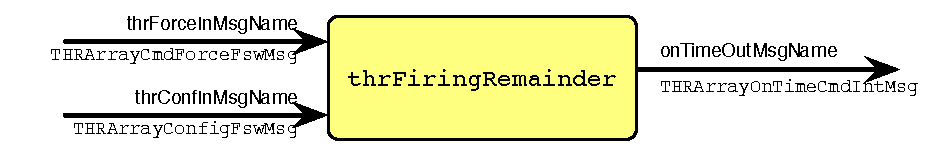
\includegraphics{Figures/moduleImg}
	}
	\caption{Illustration of the module input and output messages.}
	\label{fig:moduleImg}
\end{figure}


\section{Module Description}
This module implements a remainder tracking thruster firing logic.  More details can be found in Reference~\citenum{Alcorn:2016rz}.  

\subsection{Module Input and Output Messages}
As illustrated in Figure~\ref{fig:moduleImg}, the module reads in two messages.  One message contains the thruster configuration message from which the maximum thrust force value for each thruster is extracted and stored in the module.  This message is only read in on {\tt Reset()}.  

The second message reads in an array of requested thruster force values with every {\tt Update()} function call.  These force values $F_{i}$ can be positive if on-pulsing is requested, or negative if off-pulsing is required.  On-pulsing is used to achieve an attitude control torque onto the spacecraft by turning on a thruster.  Off-pulsing assumes a thruster is nominally on, such as with doing an extended orbit correction maneuver, and the attitude control is achieved by doing periodic off-pulsing.  

The output of the module is a message containing an array of thruster on-time requests.  If these on-times are larger than the control period, then the thruster remains on only for the control period upon which the on-criteria is reevaluated.  


\subsection{Reset() Functionality}
\begin{itemize}
	\item The control period is dynamically evaluated in the module by comparing the current time with the prior call time.  In {\tt reset()} the {\tt prevCallTime} variable is reset to 0.  
	\item The thruster configuration message is read in and the number of thrusters is stored in the module variable {\tt numThrusters}.  The maximum force per thruster is stored in {\tt maxThrust}.
	\item The on-time pulse remainder variable is reset for each thruster back to 0.0.
\end{itemize}

\subsection{Update() Functionality}
The goal of the {\tt update()} method is to read in the current attitude control thruster force message and map these into a thruster on-time output message.  Let $\Delta t_{\text{min}}$ be the minimum on-time that can be implemented with a thruster.  If the requested on-time is less than $\Delta t_{\text{min}}$, then the requested thruster on-time is clipped to zero.  In the following algorithm unimplemented fractional on-times less than $\Delta t_{\text{min}}$ are tracked and accumulated, providing additional pointing accuracy.  For example, if the minimum on-time is 20 milli-seconds, an on-time algorithm without remainder calculation would create a deadband about the 20 milli-second control request.  With the remainder logic, if 5 milli-second on-time requests are computed, these are accumulated such that every 4$^{\text{th}}$ control step a 20 milli-second burn is requested.  This reduces the deadband behavior of the thruster and achieves better pointing.  In this example the 5 milli-second un-implemented on-times are accumulated in the variable $\Delta t_{\text{partial}}$.  

If the {\tt update()} method is called for the first time after reset, then there is no knowledge of the control period $\Delta t$.  In this case the thruster on-time values are set either to 0 (on-pulsing case) or 2 seconds (off-pulsing case).  After writing out this message the module is exited.  This logic is essence turns off the thruster-based attitude control for one control period. 

If this is a repeated call of the {\tt update()} method then the control period $\Delta t$ is evaluated by differencing the current time with the prior call time.  Next a loop goes over each installed thruster to map the requested force $F_{i}$ into an on-time $t_{i}$.  The following logic is used.  
\begin{itemize}
	\item If off-pulsing is used then $F_{i}\le 0$ and we set $$F_{i} += F_{\text{max}}$$ to a reduced thrust to achieve the negative $F_{i}$ force.  
	\item Next, if $F_{i} < 0$ then it set to be equal to zero.  This can occur if an off-pulsing request is larger than the maximum thruster force magnitude $F_{\text{max}}$.  
	\item The nominal thruster on-time is computed using $$t_{i}  = \dfrac{F_{i}}{F_{\text{max}}} \Delta t$$. 
	\item If there un-implemented on-time requested $\Delta t_{\text{partial}}$ from earlier  {\tt update()} method calls, these are added to the current on-time request using $$t_{i} += \Delta t_{\text{partial}}$$ After this step the variable $\Delta t_{\text{partial}}$ is reset to 0 as the remainder calculation is stored in the on-time variable $t_{i}$.
	\item If $t_{i} < \Delta t_{\text{partial}}$ then on-time request is set to zero and the remained is set to $\Delta t_{\text{partial}} = t_{i}$
	\item If $t_{i} > \Delta $ then the requested force is larger than $F_{\text{max}}$ and the control is saturated.  In this case the on-time is set to 1.1$\Delta t$ such that the thruster remains on through the control period.
	\item The final step is to store the thruster on-time into  and write out this output message
\end{itemize}
